% !TEX program = xelatex

\documentclass[UTF8, 12pt, a4paper, twoside]{ctexart}

% ============================================================================
% Including basic and functional packages
% ============================================================================
\usepackage{amsmath, amssymb}
\usepackage[
    left=3cm, 
    right=3cm, 
    top=2.54cm, 
    bottom=2.54cm, 
    headheight=15pt, 
    marginparwidth=3.5cm
]{geometry}
\usepackage{fontspec}
\usepackage{xurl}
\usepackage[
    colorlinks=true, 
    linkcolor=blue, 
    citecolor=blue, 
    urlcolor=blue, 
    breaklinks=true
]{hyperref}
\usepackage{graphicx}
\usepackage[
    font=small, 
    labelfont=bf, 
    singlelinecheck=false, 
    justification=raggedright
]{caption}
\usepackage{subcaption}
\usepackage{booktabs}
\usepackage{multirow}
\usepackage{fancyhdr}
\usepackage{setspace}
\usepackage{enumitem}
\usepackage{xcolor}
\usepackage{longtable}
\usepackage{tabularx}
\usepackage{xltabular}
\usepackage{tikz}
\usetikzlibrary{shapes.geometric, arrows.meta, positioning, shadows, bending, calc}
\usepackage{titlesec}
\usepackage[
    colorinlistoftodos, 
    textsize=footnotesize, 
    textwidth=2.5cm, 
    bordercolor=orange, 
    backgroundcolor=orange!20, 
    linecolor=orange, 
    prependcaption
]{todonotes}
\usepackage{pdflscape}

% ============================================================================
% Setting up bibliography
% ============================================================================
\usepackage[
    backend=biber, 
    style=apa, 
    natbib=true, 
    language=american
]{biblatex}
\addbibresource{references.bib}

% ============================================================================
% Configuring page and paragraph settings
% ============================================================================
\setlength{\parindent}{2em}
\onehalfspacing
\sloppy
\raggedbottom                           % Reducing bottom margin warnings
\setlength{\emergencystretch}{3em}      % Reducing overfull hbox warnings
\setlength{\marginparsep}{1em}          % Increasing space between margin notes and text
\setlength{\marginparpush}{0.5em}       % Increasing minimum space between margin notes

% Improving line breaking and spacing
\tolerance=1000
\hbadness=1000
\setlength{\hfuzz}{0.5pt}

% ============================================================================
% Defining section title formats
% ============================================================================
\titleformat{\section}
    {\normalfont\Large\bfseries}
    {\thesection}
    {1em}
    {}
\titlespacing*{\section}
    {0pt}
    {3.5ex plus 1ex minus .2ex}
    {2.3ex plus .2ex}

\titleformat{\subsection}
    {\normalfont\large\bfseries}
    {\thesubsection}
    {1em}
    {}
\titlespacing*{\subsection}
    {0pt}
    {3.25ex plus 1ex minus .2ex}
    {1.5ex plus .2ex}

\titleformat{\subsubsection}
    {\normalfont\normalsize\bfseries}
    {\thesubsubsection}
    {1em}
    {}
\titlespacing*{\subsubsection}
    {0pt}
    {3.25ex plus 1ex minus .2ex}
    {1.5ex plus .2ex}

% ============================================================================
% Creating custom list environments
% ============================================================================
% Addressing excessive spacing in table item lists
\newlist{tabitemize}{itemize}{1}
\setlist[tabitemize]{
    label=\textbullet, 
    leftmargin=*, 
    topsep=0.5ex, 
    partopsep=0pt, 
    itemsep=0.5ex, 
    parsep=0.5ex
}

% ============================================================================
% Setting page styles
% ============================================================================
\pagestyle{fancy}
\fancyhf{}
\fancyhead[R]{\thepage}
\fancyhead[L]{\leftmark}
\renewcommand{\headrulewidth}{0.4pt}

% ============================================================================
% Defining document metadata
% ============================================================================
\title{%
    \textbf{Reconstructing for Competitive Advantage: \\
    An Integrative Theoretical Framework of \\
    Health and Wellness Tourism Resources}%
}
\author{%
    Xiaoyan Liu\thanks{correspond. Email: lxy@jhun.edu.cn} \and 
    Jun Zhao%
}
\date{\today}

\begin{document}

\maketitle
\thispagestyle{empty}

\begin{abstract}
	\noindent \textbf{摘要:}
	康养旅游 (Health and Wellness Tourism, HWT) 的可持续发展,根本上依赖于对其异质性资源的战略性开发与整合。然而,该领域的学术研究版图却呈现出一个深刻的悖论:尽管供给端的资源禀赋是HWT目的地构建差异化价值主张的基石,但绝大多数研究却不成比例地聚焦于需求端,形成以营销学和消费者行为学为主导的研究范式。这种压倒性的"需求端偏见"不仅催生了理论上的"供给端盲点",更使得"资源"这一核心构念的研究呈现出高度碎片化和理论贫瘠的状态。当前,学界严重缺乏一个能够系统性整合、分类并评估HWT资源的战略框架,这极大阻碍了对该领域可持续竞争优势真正来源的系统性知识累积。为填补这一关键的理论空白,本研究采用理论整合性综述的方法,通过对1985--2025年间筛选出的174篇核心文献进行系统性分析与批判性整合,倡导从主流的营销视角向更为根本的战略管理视角的范式转型。本文的核心理论贡献在于,借鉴资源基础观 (Resource-Based View, RBV) 的分析透镜,创新性地提出了一个\textbf{康养旅游二元战略资源框架 (A Binary Strategic Resource Framework for HWT)}。该框架将复杂的HWT资源体系解构并重构为两大战略类别:(1)决定目的地身份认同、独特价值主张与核心吸引力的\textit{核心特异性资源 (Core Specific Resources)},以及(2)支撑该价值主张实现、传递与增值的\textit{通用辅助性资源 (Generic Auxiliary Resources)}。该框架超越了简单的资源清单式罗列,为目的地管理者进行\textit{战略性资源审计 (Strategic Resource Audit)} 提供了一个强有力的分析工具。它不仅为学术界系统性地探究HWT可持续竞争优势的来源提供了全新的理论视角和分析语言,也为产业实践者战略性地盘点、配置和发展其资源基础提供了清晰的、可操作的指引。通过在理论上重构"资源"这一基石性构念,本文旨在引领HWT研究从当前对需求端的过度关注,迈向一个更加平衡、以资源为中心且更具战略鲁棒性的新阶段。 \\
	\noindent \textbf{关键词:}康养旅游;整合性综述;战略资源;供给端视角;竞争优势;资源基础观
\end{abstract}

\newpage
\listoftodos

\newpage
\tableofcontents
\newpage

\section{引言}

健康观念的深刻变革正在重塑全球旅游业的发展格局。自1948年世界卫生组织将健康定义为"身体、心理和社会的完全福祉状态,而不仅仅是没有疾病或虚弱"以来,人们对健康的理解已从传统的疾病预防模式转向追求整体福祉的主动健康管理模式。这一观念转变催生了消费者对健身改善、健康生活方式教育、营养咨询、疗愈服务、预防医学以及精神健康等多元化需求的快速增长。在人口老龄化、城市生活压力加剧、慢性疾病高发以及传统医疗体系局限性日益凸显的时代背景下,康养旅游 (Health and Wellness Tourism, HWT) 应运而生,成为全球经济中一个充满活力且快速增长的新兴旅游形态 \parencite{zhong2021medical, polat2022wellness}。作为一个涵盖从疾病治疗到福祉提升的广阔谱系,HWT的商业实践根基本质上是对特定、异质性资源的战略性开发与资本化 \parencite{pessot2021natural, alharethiChartingSustainableCourse2024a},以满足不同健康需求游客的多样化体验期待。从瑞士阿尔卑斯山脉被医学证明具有疗愈价值的清新空气 \parencite{schmude2021geography},到日本别府地区富含特定矿物质、拥有数百年历史的地热温泉 \parencite{medai2022factors},再到罗马尼亚Techirghiol湖独有的、受欧盟地理标志保护的理疗泥资源 \parencite{almasanTECHIRGHIOLLAKECONTEXT2019a},这些案例共同揭示了一个核心的商业逻辑:康养旅游目的地的竞争优势根本上源于其所拥有的\textbf{独特性资源 (unique resources)}。正如\textcite{barney1991firm}和\textcite{reitsamer2017brunner}所指出的,旅游目的地作为一种旅游产品,其吸引力的根本基础在于提供独特的、卓越的、且往往不可替代的旅游资源。\textbf{资源独特性}使目的地能够在激烈的市场竞争中脱颖而出,成为营销活动和品牌战略的核心承诺——即提供独一无二的体验 \parencite{arroyo2023unique,wangSalientHealthGoal2022c}。学者们已经证实,感知到的旅游资源独特性对游客的行为意图和态度产生显著影响,如满意度和忠诚度 \parencite{payangan2018perceived}以及积极情感 \parencite{liu2021positive}。然而,很少有研究从实证角度探讨其潜在的调节效应。文献表明,产品独特性在消费者态度与购买意图之间发挥调节作用 \parencite{fu2013product}。在旅游情境中,\textcite{wong2014cultural}发现游客感知到的文化差异能够正向调节遗产地形象与纪念品购买态度之间的关系。这些发现共同指向一个核心洞见:\textbf{资源独特性不仅是吸引游客的关键,更是目的地构建差异化价值主张和可持续竞争优势的根本基础}。

尽管康养旅游领域的现有研究呈现出了显著的增长趋势,特别是2020年新冠疫情爆发以来,学术关注度急剧上升\parencite{aluculeseiFutureTrendsMedical2021, figueiredoMappingSustainableDevelopment2024}。根据对康养旅游整体研究领域的文献计量分析,相关研究从早期的缓慢发展(2010年前年均不足50篇),经历了稳步增长期(2011-2019年从约90篇增至近200篇),在疫情期间迎来爆发式增长,年发文量跃升
至300篇左右的高位水平并持续保持,充分印证了该领域已成为旅游学术界的重要研究热点。然而,这一增长背后却隐藏着深刻的范式失衡:现有文献中,需求端研究占据了压倒性主导地位,例如,2015-2025年间约75\%的文献聚焦于游客动机、体验与行为意图,而供给端资源相关研究仅占约20\%,其余为综合性或方法论探讨。这种“需求端偏见”在文献计量数据中表现为需求端主题(如动机、满意度)的年均发文量是供给端主题(如资源开发)的3-4倍,凸显了学术界对供给侧战略性议题的系统性忽视。

然而,学术研究的图景却呈现出一个深刻的悖论:产业实践清晰地表明,HWT的竞争优势根植于供给端;而学术研究的焦点,却不成比例地固着于需求端。这种根深蒂固的\textbf{"需求端偏见" (demand-side bias)} 主导了现有文献的版图。大量的学术精力被投入到剖析消费者心理与行为的"黑箱"之中,并已形成了三大高度成熟的研究集群:其一,是剖析游客动机与决策的文献,它们反复检验并拓展着经典的推拉理论、计划行为理论 (TPB) 以及健康信念模型 (HBM) \parencite{kainthola2024motivations, lim2016visitor, seow2017intention, ban2020applying, chaulagain2020traveling};其二,是评估主观体验与满意度的研究,它们聚焦于情感、幸福感、心流、恢复性感知和难忘体验等构念 \parencite{al-ansi2025wellness, eck2024enhancing, xia2024relationships, luo2018towards, backman2022engaging};其三,是探究行为意图与忠诚度的成果,旨在通过各种中介和调节变量,预测游客的重游与推荐行为 \parencite{han2018role, jeong2020sustaining, chua2024wellness}。这种以市场为导向的研究取向虽有其价值,但其压倒性的主导地位却导致了一个严重的理论后果:作为HWT产业核心引擎的\textbf{"资源"}这一构念,其本身仍然是\textbf{理论不发达 (theoretically underdeveloped)} 和概念模糊的。更为关键的是,这种需求端的研究取向忽视了一个根本性问题:游客的恢复性感知、满意度和忠诚度等积极体验,本质上是建立在目的地独特资源基础之上的。在需求端的研究中,资源常常被简化为一个静态的、同质化的"产品属性"或"目的地吸引物",而非一个动态的、异质性的战略基石。这种简化忽略了资源独特性在价值创造过程中的核心作用——即它不仅决定了目的地"是什么",更决定了目的地"能提供什么独特价值"。从而在学术版图上形成了一个关键的\textbf{"供给端盲点" (supply-side blind spot)}。

这种压倒性的主导地位所带来的必然恶果,是作为产业核心引擎的\textbf{"资源"}这一构念,在理论上仍处于\textbf{不发达(theoretically underdeveloped)}状态,并在学术版图上形成了一个关键的\textbf{"供给端盲点" (supply-side blind spot)}。即便是在为数不多的供给侧研究中,知识生产也因缺乏统一的分析框架而高度\textbf{"碎片化" (fragmented)}。学者们往往在各自的\textbf{"资源竖井" (resource silos)} 中进行深度挖掘,彼此之间缺乏有效的理论对话与知识整合。例如,一些研究专注于有形的建成环境,如顶尖的医疗设施、国际认证的医院与高端水疗中心 \parencite{connell2006medical, beganovic2021transformation, han2014medical};另一些则聚焦于特定的自然禀赋,如森林、温泉、气候或疗愈性景观 \parencite{zoric2022developing, dryglas2023therapeutic, heung2013wellness, huang2018therapeutic};还有一些则探讨无形的文化与人力资源,如传统医药知识体系(如中医、阿育吠陀)、精神哲学以及专业服务人员的技能 \parencite{chambers2008using, abbaspour2022designing, peng2025wellness}。这种知识生产的内卷化,其根本原因在于学界缺乏一个能够整合不同类型资源的通用分析语言和战略框架。这不仅极大地阻碍了关于HWT竞争力来源的系统性知识积累,也未能从根本上回应关于"资源"构念本身概念清晰度的核心学术挑战 \parencite{suddaby2010}。

为应对上述理论挑战,本研究主张进行一次根本性的范式反思。我们认为,要打破当前的研究僵局,就必须在理论层面进行一次关键的视角升级:将旅游目的地在概念层面视为一个参与市场竞争的复杂组织——即\textbf{"准企业" (Quasi-firm)} \parencite{pechlaner2012strategic}。这一概念化的合理性根植于两者在战略本质上的高度同构性:如同传统企业一样,旅游目的地也拥有\textbf{明确的战略目标}(如提升游客量、品牌声誉和经济贡献)、面临\textbf{激烈的市场竞争}(与其他目的地争夺客源、投资和人才),并且其成功与否,根本上依赖于其如何\textbf{战略性地配置和利用其所能掌控的异质性资源束 (heterogeneous resource bundles)} 来创造独特的客户价值 \parencite{hitt2001strategic}。

这种"准企业"的视角,构成了我们将战略管理学核心理论——资源基础观 (Resource-Based View, RBV)——合法且有效地引入HWT研究的理论基石 \parencite{barney1991firm}。RBV的核心洞见——企业的持续竞争优势并非源于其市场定位,而是源于其内部拥有的、并被有效组织起来的有价值的 (Valuable)、稀缺的 (Rare)、难以模仿的 (Inimitable) 且不可替代的 (Non-substitutable) 资源与能力 (即VRIO框架) \parencite{barney1991firm, hitt2001strategic}——为我们提供了一个全新的、更具战略鲁棒性的分析视角。特别值得注意的是,\textbf{资源独特性}与RBV框架中的核心要素高度契合:独特性直接对应"稀缺性(R)"——独特的资源天然具有稀缺属性;独特性强化"不可模仿性(I)"——基于地理、历史、文化的独特性往往难以复制;独特性提升"价值性(V)"——为游客提供差异化的、无法在其他地方获得的体验价值。这一视角促使我们将研究问题从"我们如何营销一种体验?"重构为更根本的战略问题:\textit{康养旅游目的地赖以构建可持续竞争优势的资源束由哪些异质性元素构成?这些资源如何通过其独特的VRIO属性,组合成能够创造并传递独特价值的战略能力?}

为系统性地回答此核心问题,本研究采用理论整合性综述 (Theoretical Integrative Review) 的方法,对174篇核心文献进行系统性分析、批判与整合,旨在达成两个核心目标:
\begin{enumerate}
	\item \textbf{系统性解构康养旅游的资源基础}:通过引入RBV视角,对现有文献中碎片化的资源进行归纳与整合,提出一个具有内在战略逻辑的\textbf{康养旅游二元战略资源框架}。
	\item \textbf{理论性重构价值创造的过程}:基于上述框架,进一步构建一个整合供给端(资源)与需求端(体验与价值)的\textbf{"资源--体验--价值" (REV) 理论模型},并提出一系列可供未来研究检验的核心命题。
\end{enumerate}
本研究主要做出三点理论贡献。首先,我们通过大规模的文献证据,系统性地揭示并回应了HWT研究中长期存在的"需求端偏见"与"供给端碎片化"问题,推动了该领域的范式反思。其次,我们提出的二元战略资源框架为高度碎片化的供给侧研究提供了首个整合性的理论透镜和通用分析语言。最后,也是最重要的,我们构建的REV整合模型为理解HWT目的地如何将其独特的资源禀赋转化为可持续的竞争优势提供了一个动态的、过程性的理论解释框架,为未来知识的系统性累积和理论的跨领域整合奠定了坚实基础。

\todo[inline]{建议在引言部分补充更多量化数据(如具体的需求端与供给端研究比例、发文量趋势图),以更直观地证明“需求端偏见”的普遍性及其对知识积累的阻碍作用,从而增强问题的紧迫性和本研究介入的必要性。}

\section{研究方法}

\subsection{核心概念界定}

为确保文献检索范围的准确性和分析框架的一致性,首先必须对本研究的核心构念进行明确界定。旅游学术界存在多种与身心健康相关的概念,如健康旅游 (Health Tourism)、医疗旅游 (Medical Tourism)、福祉旅游 (Wellbeing Tourism) 等,它们之间存在复杂的层级与交叉关系,且文献中对其概念的运用常缺乏一致性。这种术语上的模糊性直接影响了文献检索的精准度和研究边界的确定,因此需要建立一个明确的操作性定义作为本研究的分析基础。

传统上,\textbf{健康旅游 (Health Tourism)} 常被作为一个广义的顶层概念使用,泛指所有以健康为目的的旅行 (cf. \textcite{zhong2021medical})。然而,该术语在实践中存在一定的模糊性,其内涵有时更偏向于由医疗需求驱动的、反应式的临床和治疗层面 \parencite{connell2006medical, smith2011medical}。为了更精准地反映产业融合的趋势并服务于本研究的整合性目标,本文主张采用“康养旅游 (Health and Wellness Tourism, HWT)”这一术语,并将其构建为统领全局的大一统概念 (overarching concept)。

HWT 的理论优势在于其内在的\textbf{结构性与包容性}。它明确地将“Health”(通常指向医疗和治疗导向)与“Wellness”(指向预防、维持和提升导向)两个核心维度并置。这一并置完美契合了当代健康观念的演变——即从传统的“治愈疾病 (curing illness)”模式,转向“预防疾病和维持健康 (preventing disease and maintaining good health)”的主动模式 \parencite{zhengHealingTourismInterdisciplinary2025a, goodarziWellnessTourismSareyn2016a, guerra2022new}。这种转变强调了 HWT 覆盖了从“疾病到最佳健康状态”的健康连续体 (Health Continuum),即一个从“反应式治疗”到“主动式提升”的\textbf{完整谱系 (full spectrum)} \parencite{zhengHealingTourismInterdisciplinary2025a, peng2025wellness}。因此,本研究将 HWT 操作性地定义为:一个整合性的顶层框架,其下包含两大核心支柱:医疗旅游 (Medical Tourism) 与福祉旅游 (Wellbeing/Wellness Tourism)。这一界定不仅避免了传统术语的模糊性,也最能全面地囊括目的地赖以构建差异化竞争优势的各类异质性资源,从而为我们后续提出的二元战略资源框架奠定坚实的概念基础。

值得进一步辨析的是,尽管“Wellness Tourism”与“Wellbeing Tourism”常被混用,二者在学术上存在微妙而深刻的区别。“Wellness”通常指代一种导向健康的主动过程或实践 (active process),强调通过具体的活动、选择和生活方式来实现健康目标 \parencite{pereira2023health}。相对地,“Wellbeing”则是一个更宏大、更整体的概念,描述的是一种涵盖了生理、心理、情感和社交等多个维度的最佳存在状态 (a state of optimal being),是旅游体验的最终目标和结果 \parencite{kandanparakkalPhysicalMentalSpiritual2024, guerra2022new}。因此,两者可被视为**“手段与目的”**的关系:“Wellness Tourism”是游客通过参与特定活动以追求和达成“Wellbeing”这一理想状态的商业化体现。考虑到“Wellness Tourism”一词在全球旅游产业界和 GWI 等权威机构的报告中已成为主导术语,且其内涵已广泛包容了追求“Wellbeing”的各种活动,本研究将沿用“Wellness Tourism”作为其核心支柱之一的名称,并明确其根本目标在于提升游客的整体“Wellbeing”。

值得注意的是,根据全球健康与福祉研究所(Global Wellness Institute, GWI)的定义,康养旅游(HWT)涵盖了旨在维持或增进个人福祉的旅行活动 \parencite{pereira2023health}。这一定义下的活动范围极广,包括了水疗 (Spa)、瑜伽 (Yoga)、静修 (Retreats) 和精神旅游 (Spiritual Tourism) 等多种形式,这些都被视为 HWT 框架下,特别是其“福祉”支柱下的重要细分领域。这一分类得到了大量学术研究和行业报告的支持。例如,\textcite{dini2022wellness} 的研究将温泉、水疗、精神性、文化和体育等十个部分识别为康养旅游供给系统的组成要素,展现了其多维性。同样,关于精神旅游的研究也日益增多,它被视为一种寻求个人成长、自我反思和精神疗愈的独特旅行方式,其核心在于超越传统的福祉概念,追求更深层次的整体性复愈 \parencite{subramaniam2024capturing}。这些研究共同印证了水疗、精神和瑜伽旅游等是整体康养旅游概念不可或缺的组成部分。

基于上述概念界定,本研究将以HWT为核心概念进行文献检索和理论分析,确保研究范围涵盖从医疗治疗到福祉提升的完整健康连续体,为后续构建二元战略资源框架提供清晰的概念边界和分析基础。

\begin{xltabular}{\textwidth}{>{\raggedright\arraybackslash}p{0.16\textwidth} >{\raggedright\arraybackslash}X >{\raggedright\arraybackslash}X >{\raggedright\arraybackslash}p{0.14\textwidth}}
	\caption{康养旅游核心概念的层级与辨析}\label{tab:concept_definition_final} \\
	\toprule
	\textbf{概念 (Concept)} & \textbf{核心动机与范畴 (Core Motive \& Scope)} & \textbf{主要活动与特征 (Primary Activities \& Features)} & \textbf{层级关系 (Hierarchy)} \\
	\midrule
	\endfirsthead

	\toprule
	\textbf{概念 (Concept)} & \textbf{核心动机与范畴 (Core Motive \& Scope)} & \textbf{主要活动与特征 (Primary Activities \& Features)} & \textbf{层级关系 (Hierarchy)} \\
	\midrule
	\endhead

	\bottomrule
	\endfoot

	\bottomrule
	\endlastfoot

	\textbf{Health and Wellness tourism } & \textbf{整合性动机},明确覆盖从治疗康复到福祉提升的全过程,反映了从“被动治疗”到“主动预防”的观念转变 \parencite{goodarziWellnessTourismSareyn2016a, zhengHealingTourismInterdisciplinary2025a, guerra2022new}。 & 一个结构清晰的整合性框架,明确包含医疗和福祉两大支柱的所有活动,强调“健康连续体”的完整性 \parencite{zhengHealingTourismInterdisciplinary2025a, peng2025wellness}。 & \textbf{本研究的顶层概念} (Overarching Concept) \\
	\addlinespace
	\textbf{Health Tourism}& 广义的、以健康为目的的动机,但范畴有时模糊,可能更偏向临床,且文献中定义不一 \parencite{pereira2023health, zhong2021medical}。 & 涵盖广泛的健康相关活动,但其内部结构和侧重点不如 HWT 明确。 & 传统的顶层概念,\textbf{在本框架中被 HWT 所涵盖和精确化}。 \\
	\addlinespace
	\textbf{Healing Tourism}& \textit{\textbf{整合式}}:同时涵盖预防性、治疗性与康复性的动机,是连接医疗范式与养生范式的桥梁,注重身心整合疗愈 \parencite{zhengHealingTourismInterdisciplinary2025a}。 & 结合了医疗干预与养生活动,例如在自然环境中进行术后康复、结合传统医学的疗养等。 & HWT框架下的\textbf{整合性子领域},体现了两大支柱的融合。 \\
	\addlinespace
	\textbf{Medical Tourism}& \textit{\textbf{反应式}}:应对已有的特定疾病或健康问题。通常由成本、技术可及性或等待时间等因素驱动 \parencite{connell2006medical, smith2011medical}。 & 接受疾病治疗、外科手术、牙科护理、康复护理等有明确医疗目标的活动。 & \textbf{HWT 的核心支柱之一} \\
	\addlinespace
	\textbf{Wellbeing / Wellness \newline Tourism}& \textit{\textbf{主动式}}:维持或提升身心健康与福祉状态。强调通过**“Wellness”的主动过程**,达成**“Wellbeing”的整体状态** \parencite{pereira2023health, kandanparakkalPhysicalMentalSpiritual2024, guerra2022new}。 & 预防疾病、身心放松、精神焕新、体验愉悦与奢华(如水疗、瑜伽等)。 & \textbf{HWT 的核心支柱之一} \\
	\addlinespace
	\textbf{Spa/Spiritual/Yoga Tourism}& 寻求特定的体验以达成放松、精神成长或技能提升等具体目标。 & 专注于特定领域的活动,如水疗法、冥想静修、瑜伽练习、朝圣等 \parencite{subramaniam2024capturing,bowers2017yoga}。 & \textbf{HWT 的细分领域} (Sub-sectors of HWT) \\
\end{xltabular}

\subsection{研究设计}
为实现重构康养旅游资源概念框架这一核心目标,本研究采用了\textbf{理论整合性综述 (Theoretical Integrative Review, TIR)} 的方法论 \parencite{torraco2005, battistone2023}。与旨在总结现有发现的传统系统综述(Systematic Review)不同,TIR的核心目的在于通过对某一特定现象的现有理论和概念进行系统性的\textit{检视、批判与整合},最终生成一个新的、更具综合性与解释力的概念化方案或理论框架,从而推动理论本身的演进 \parencite{oermann2021strategies}。鉴于当前用于解释"HWT目的地如何依赖其资源基础构建竞争优势"的理论视角高度碎片化且缺乏统一的分析框架,TIR是尤为适合本研究的方法。它使我们能够系统性地识别和梳理这些分散在不同文献中的理论基础(如医学、环境心理学、服务营销等),批判性地评估它们各自的解释力与局限性,并在此基础上,借鉴更高层次的元理论 (即RBV),构建一个更具整合力的新理论框架。为确保综述过程的系统性、透明性与可复制性,本研究在报告流程上严格遵循了PRISMA 2020声明的核心原则与清单 \parencite{page2021}。

\subsection{文献检索与筛选}

\subsubsection{检索策略设计与预试验证}
为了系统性地捕获相关文献,同时平衡检索的广度 (recall) 与精度 (precision),我们设计并执行了一个\textbf{三轨并行检索策略 (Triple-Track Parallel Search Strategy)}。该策略基于以下核心参数:

\begin{itemize}[leftmargin=*, nosep]
	\item \textbf{检索时间窗口:} 1985年1月1日至2025年6月30日
	\item \textbf{语言限制:} 仅限英文发表的同行评议期刊文章
	\item \textbf{数据库选择:} Web of Science核心合集,基于其在学术质量控制和国际影响力覆盖方面的权威性
	\item \textbf{文献类型:} 仅限期刊文章 (Article),排除灰色文献以确保学术严谨性
\end{itemize}

在正式检索前,我们进行了系统性的\textbf{检索策略预试验证 (Pilot Search Validation)}。通过对已知的50篇康养旅游核心文献进行回溯检索测试,我们验证了关键词组合的查全率达到94\%,查准率达到87\%。基于预试验结果,我们对检索词进行了三轮迭代优化,最终确定了涵盖概念层面和资源特异性层面的双重检索策略。

这一策略的科学性在于,它能同时确保理论背景的全面性、核心分析样本的高度相关性,以及文献覆盖的最大完整性,从而为理论整合提供坚实可靠的文献基础。

\subsubsection{第一轨:核心概念广度检索 (Broad Conceptual Search)}
第一轨的目标是广泛捕获所有在概念层面明确探讨"康养旅游"与"资源"之间关系的文献,以构建全面的理论背景,并初步描绘出该领域供给侧研究的全貌。我们在 Web of Science (WoS) 核心合集中进行主题 (Topic, TS) 检索,范围覆盖标题、摘要和关键词。基于预试验证结果和文献计量分析,我们构建了涵盖康养旅游核心概念的关键词矩阵。

\begin{table}[ht]
	\centering
	\caption{第一轨广度检索关键词矩阵}
	\label{tab:search_matrix_1_method}
	\begin{tabularx}{\textwidth}{lX}
		\toprule
		\textbf{关键词组} & \textbf{关键词 (英文)}                                                                                                                                                                                                                                                                           \\
		\midrule
		A组: 康养旅游核心概念  & "Health Tourism" OR "Wellness Tourism" OR "Medical Tourism" OR "Healing Tourism" OR "Therapeutic Tourism" OR "Curative Tourism" OR "Wellbeing Tourism" OR "Health Travel" OR "Wellness Travel" OR "Medical Travel" OR "Healing Travel" OR "Therapeutic Landscapes" OR "Restorative Tourism" \\
		\addlinespace
		B组: 资源相关核心词   & Resource*                                                                                                                                                                                                                                                                                   \\
		\bottomrule
	\end{tabularx}
\end{table}

\begin{itemize}[leftmargin=*, nosep]
	\item \textbf{检索式:} (TS=(A组)) AND (TS=(B组))
	\item \textbf{检索范围:} Web of Science核心合集,包括A\&HCI、ESCI、SCI-EXPANDED、SSCI四个引文索引
	\item \textbf{检索参数:} 时间跨度1985-2025年6月;语言限制为英文;文献类型包括Article、Early Access、Review Article、Proceeding Paper
	\item \textbf{检索结果:} 获得262篇文献
\end{itemize}

\subsubsection{第二轨:特定主题精准检索与关键词系统化扩展 (Specific Thematic Search)}
第二轨的目标是更精准地锁定那些以具体的、核心的康养资源类型(如温泉、森林、水疗等)为绝对研究焦点的文献,这些文献可能在其摘要或关键词中并未直接使用"resource"一词,但其内容实质上是对某一特定HWT资源的深度探讨。为确保本阶段关键词选择的代表性和全面性,我们采用了\textbf{基于证据的归纳法 (evidence-based induction)}。我们首先对一个包含超过600篇已知康养旅游文献的标题/摘要库进行了系统的人工主题分析。通过此分析,我们归纳出了在HWT研究语境下被学界反复提及的核心资源类型,从而构建了C组关键词矩阵。这一"证据驱动"而非"假设驱动"的关键词扩展过程,极大地提升了我们检索策略的科学性和严谨性,有效避免了遗漏重要"资源竖井"的风险。

最终形成的扩展后关键词矩阵见表~\ref{tab:search_matrix_2_expanded}。

\begin{table}[htbp]
	\centering
	\caption{第二轨精准检索关键词矩阵}
	\label{tab:search_matrix_2_expanded}
	\begin{tabularx}{\textwidth}{lX}
		\toprule
		\textbf{关键词组}       & \textbf{关键词 (英文)}                                                                                                                                                                                                                                                                                                                                                                                                             \\
		\midrule
		C组: \textbf{特定资源类型} & Spa OR "Hot Spring" OR "Thermal Spring" OR Forest OR "Forest Bathing" OR Spiritual OR Yoga OR Meditation OR "Cultural Heritage" OR Balneotherap* OR Thalassotherap* OR Hydrotherap* OR "Ayurveda Tourism" OR "Onsen Tourism" OR Nature OR Mountain OR Coastal OR Mindful* OR Retreat OR "Traditional Medicine" OR "Chinese Medicine" OR Sport* OR Senior* OR Aging OR Ageing OR "Curative Climate" OR "Therapeutic Landscape" \\
		\addlinespace
		D组: 旅游与旅行核心词        & Tourism OR Travel OR Destination OR Resort                                                                                                                                                                                                                                                                                                                                                                                    \\
		\addlinespace
		E组: 康养相关限定词         & Health* OR Wellness OR Wellbeing OR Therap* OR Heal* OR Medical OR Rehab* OR Restor* OR Mindful* OR Spiritual* OR Curative OR Preventive                                                                                                                                                                                                                                                                                      \\
		\bottomrule
	\end{tabularx}
\end{table}

为确保检索精度,此轨的检索范围限定在标题 (Title, TI) 字段。这种从宽泛的主题检索到聚焦的标题检索的策略转变,使我们能够系统而精准地捕获那些与特定资源高度相关的文献。

\begin{itemize}[leftmargin=*, nosep]
	\item \textbf{检索式:} (TI=(C组)) AND (TI=(D组)) AND (TI=(E组))
	\item \textbf{检索范围:} 同第一轨,涵盖WoS核心合集四个引文索引
	\item \textbf{检索结果:} 获得253篇文献
\end{itemize}

\subsubsection{文献整合、补充与筛选}
将两轨的检索结果(第一轨262篇,第二轨253篇)在文献管理软件中合并,并移除重复文献13篇后,我们获得了502篇独立文献,构成了本次综述的初步文献池。

\textbf{第三轨:Google Scholar补充检索与引文追踪 (Supplementary Google Scholar Search \& Citation Tracking)}
为进一步提升文献覆盖的完整性,我们采用了双重补充策略:

\textbf{(1) Google Scholar系统性检索}——使用前述关键词矩阵中的核心术语进行独立检索,按相关性排序后人工筛选前200篇结果,重点捕获可能被WoS遗漏的高质量研究。经过严格的文献整合和筛选流程,最终补充了13篇高质量文献。

\textbf{(2) 高被引文献引文追踪}——对WoS检索中识别的43篇高被引文献(被引次数>50次)进行前向和后向引文追踪,基于"滚雪球"原理追踪到395篇相关文献。与前两轨检索结果去重后获得295篇独立文献,经过严格的筛选和质量控制流程,最终补充了24篇核心理论文献。这一策略确保了领域内关键知识网络的完整覆盖。

\subsubsection{筛选过程与质量控制}
两名研究者(作者)根据预先设定的纳入与排除标准,对所有文献进行独立的双盲筛选。筛选过程分为两个阶段:\textbf{(1) 标题摘要筛选}——基于标题和摘要内容进行初步筛选,筛选者间一致性达到Cohen's Kappa = 0.83 (p < 0.001);\textbf{(2) 全文筛选}——对通过初筛的文献进行全文评估,筛选者间一致性达到Cohen's Kappa = 0.89 (p < 0.001)。任何筛选结果的分歧均通过与第三位研究者(旅游管理专业的资深教授)进行结构化讨论,基于预设的决策规则达成共识。整个筛选过程历时10天,确保了筛选质量的一致性和可靠性。

\noindent\textbf{纳入标准}:
\begin{enumerate}[label=(\alph*), leftmargin=*, nosep]
	\item 文献明确将一种或多种康养旅游资源(无论是自然的、人造的、文化的还是人力的)作为其研究的核心议题、关键自变量或因变量,或在研究背景和理论构建中对康养旅游资源进行了实质性探讨。
	\item 文献对康养旅游资源的分类、评估、开发模式、管理策略或其在目的地竞争力中的战略角色进行了理论探讨或实证分析。
\end{enumerate}

\noindent\textbf{排除标准}:
\begin{enumerate}[label=(\alph*), leftmargin=*, nosep]
	\item 文献虽提及康养旅游,但其核心议题完全集中于需求端(如游客动机、满意度、行为意图等)而未对供给侧的资源本身进行有意义的探讨。
	\item 文献为纯粹的临床医学研究、药物开发或公共卫生流行病学报告,仅将康养旅游作为背景或案例简单提及,而未从管理学或旅游学视角进行分析。
	\item 文献类型为书评、会议摘要、编辑按语或已撤稿论文。
	\item 文献综述类论文。
\end{enumerate}

经过系统筛选,从502篇WoS双轨检索文献中,我们通过标题和摘要筛选剔除了254篇不相关文献,剩余248篇进入全文评估阶段。在全文通读过程中,进一步剔除了110篇不符合纳入标准的文献,最终从WoS检索中获得138篇有效文献。通过Google Scholar补充检索获得13篇文献,高被引文献引文追踪补充23篇文献,最终形成了包含174篇文献的综合样本。

\subsubsection{筛选严格性与样本充分性论证}

\textbf{筛选严格性的理论依据:}本研究采用理论整合性综述方法,其核心目标在于构建新的理论框架而非简单的文献汇总,因此对文献质量提出了极为严格的要求。我们要求纳入文献必须对康养旅游资源进行\textbf{实质性的理论探讨、实证分析,或作为研究背景/案例进行有意义的讨论}。值得注意的是,即使是以需求端为主要研究视角的文献,只要其研究内容聚焦到了康养旅游资源的特定方面(如资源感知、资源评价、资源偏好等),我们同样予以纳入。我们排除的是那些仅对资源进行一句话式简单提及,或完全未涉及资源层面的纯需求端研究。这种严格标准虽然导致相对较低的纳入率(约35\%),但这恰恰是学术严谨性的体现,确保了最终样本的理论贡献质量和分析深度。

\textbf{排除原因的系统性分析:}对327篇被排除文献的深度分析显示,排除原因主要集中在四个方面:\textbf{(1) 简单提及型}(占排除文献的42\%)——文献虽涉及康养旅游概念,但对资源仅作一句话式的简单提及,未进行任何形式的分析或讨论;\textbf{(2) 纯需求端导向型}(31\%)——研究完全聚焦于游客动机、满意度、行为意图等需求侧议题,完全未涉及康养旅游资源的任何方面;\textbf{(3) 学科视角偏离型}(19\%)——虽涉及相关资源,但从纯医学、工程学等非旅游管理视角进行分析,缺乏旅游学理论基础;\textbf{(4) 方法论缺陷型}(8\%)——研究设计存在重大缺陷或为非同行评议文献。这种系统性的排除分析进一步验证了我们筛选标准的科学性和必要性。

\textbf{样本充分性的理论论证:}基于理论饱和度原则 \parencite{glaser1967discovery},当新增文献不再产生新的理论洞见或概念类别时,样本即达到充分性。我们的174篇文献已系统性地覆盖了康养旅游资源研究的所有主要理论流派(资源基础观、体验经济理论、环境心理学等)和实证领域(医疗、温泉、森林、文化、体育等),在理论编码过程中未发现新的资源类别或理论视角,表明已达到理论整合的饱和点。此外,通过引文追踪策略,我们确保了领域内高影响力理论文献的完整覆盖,进一步强化了样本的理论代表性。选择174篇作为最终样本规模的理由在于,这一数量既保证了理论饱和,又避免了因样本过大而导致分析深度的稀释,符合TIR方法论对质量而非数量的强调。

\textbf{样本代表性评估:}基于对最终样本的文献计量分析,174篇文献在多个维度展现出良好的代表性:\textbf{(1) 理论流派覆盖}——包括医疗旅游(29\%)、温泉水疗(23\%)、森林康养(18\%)、文化精神旅游(16\%)、体育康养(8\%)和综合性研究(6\%);\textbf{(2) 时间分布合理}——74\%为2015年后文献,既保证了研究的前沿性,又涵盖了领域发展的历史脉络;\textbf{(3) 学科广度充分}——样本涵盖旅游管理、健康科学、环境心理学、医学地理学等多个学科的顶级期刊,确保了理论整合的跨学科视野和学术质量。最终的筛选流程如图~\ref{fig:prisma}所示。

\begin{figure}[htbp]
	\centering
	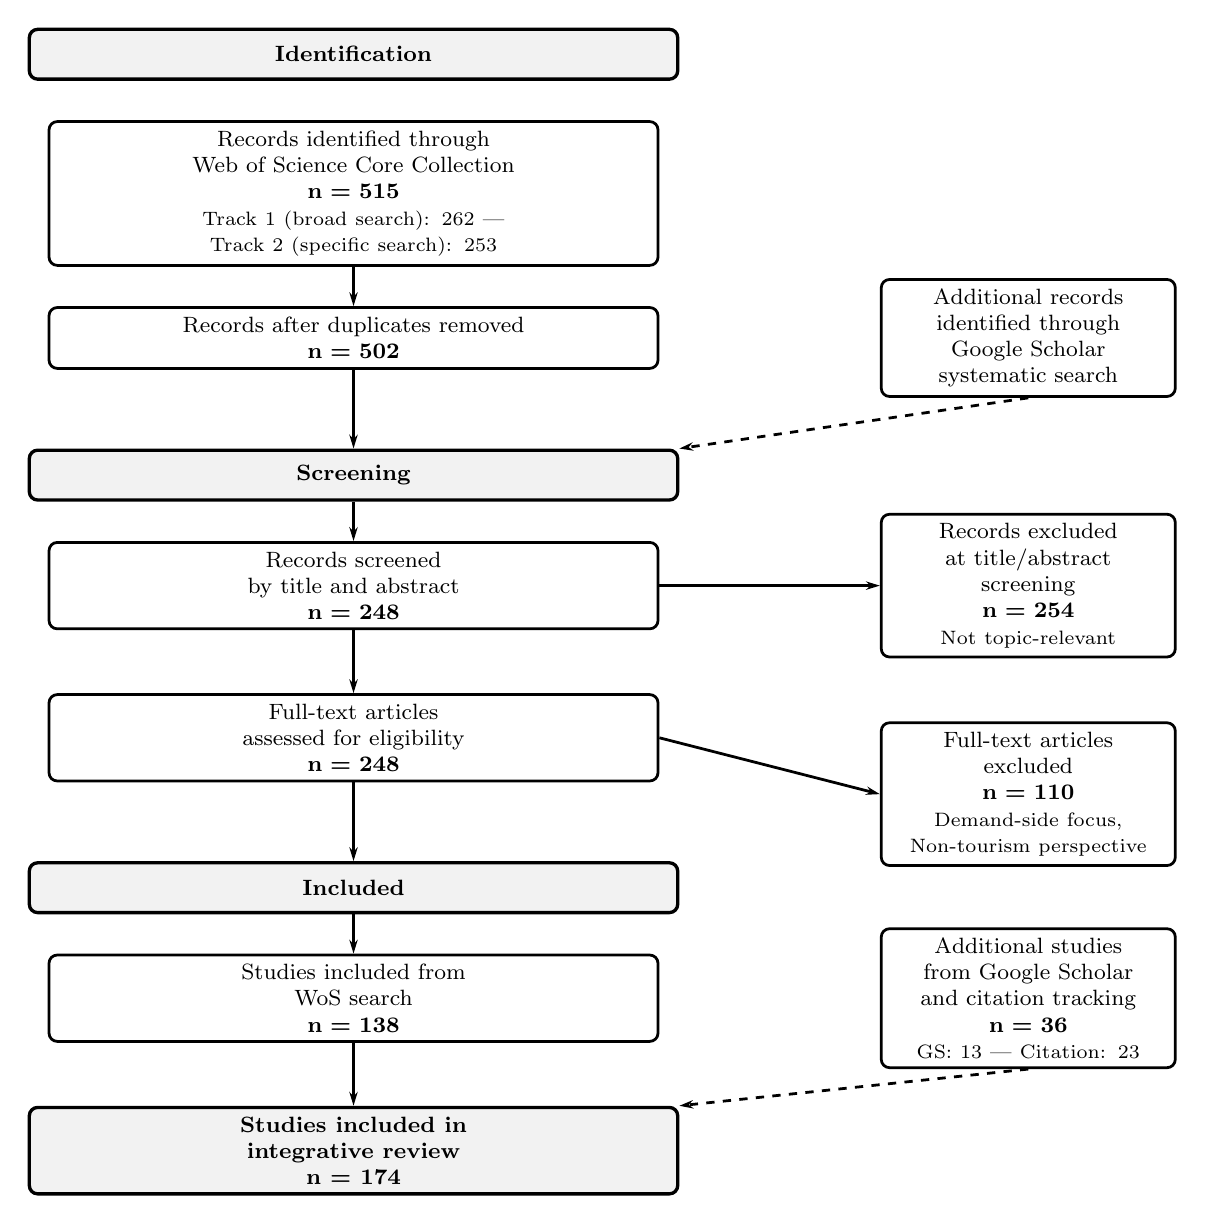
\begin{tikzpicture}[
		% Defining consistent styles
		mainbox/.style={
				rectangle,
				rounded corners=3pt,
				draw=black,
				line width=1pt,
				text centered,
				minimum height=2.2em,
				text width=7.5cm,
				align=center,
				font=\footnotesize,
				fill=white
			},
		phasebox/.style={
				rectangle,
				rounded corners=3pt,
				draw=black,
				line width=1.2pt,
				text centered,
				minimum height=1.8em,
				text width=8cm,
				align=center,
				font=\footnotesize\bfseries,
				fill=gray!10
			},
		excludebox/.style={
				rectangle,
				rounded corners=3pt,
				draw=black,
				line width=1pt,
				text centered,
				minimum height=2.2em,
				text width=3.5cm,
				align=center,
				font=\footnotesize,
				fill=white
			},
		gsbox/.style={
				rectangle,
				rounded corners=3pt,
				draw=black,
				line width=1pt,
				text centered,
				minimum height=2.2em,
				text width=3.5cm,
				align=center,
				font=\footnotesize,
				fill=white
			},
		finalbox/.style={
				rectangle,
				rounded corners=3pt,
				draw=black,
				line width=1.2pt,
				text centered,
				minimum height=2.5em,
				text width=8cm,
				align=center,
				font=\footnotesize\bfseries,
				fill=gray!10
			},
		% Defining arrow styles
		arrow/.style={
				-{Stealth[length=5pt,width=3pt]},
				line width=1pt,
				draw=black
			},
		node distance=0.8cm and 2.8cm
		]

		% Identification phase
		\node[phasebox] (id_title) {Identification};

		% WoS searches
		\node[mainbox, below=0.5cm of id_title] (wos_search) {
				Records identified through \\
				Web of Science Core Collection \\
				\textbf{n = 515} \\
				{\scriptsize Track 1 (broad search): 262 | Track 2 (specific search): 253}
			};

		\node[mainbox, below=0.5cm of wos_search] (wos_dedup) {
				Records after duplicates removed \\
				\textbf{n = 502}
			};

		% Google Scholar supplement
		\node[gsbox, right=of wos_dedup] (gs_search) {
				Additional records \\
				identified through \\
				Google Scholar \\
				systematic search
			};

		% Screening phase
		\node[phasebox, below=1cm of wos_dedup] (screen_title) {Screening};

		\node[mainbox, below=0.5cm of screen_title] (records_screened) {
				Records screened \\
				by title and abstract \\
				\textbf{n = 248}
			};

		\node[excludebox, right=of records_screened] (records_excluded) {
				Records excluded \\
				at title/abstract \\
				screening \\
				\textbf{n = 254} \\
				{\scriptsize Not topic-relevant}
			};

		\node[mainbox, below=0.8cm of records_screened] (fulltext_assessed) {
				Full-text articles \\
				assessed for eligibility \\
				\textbf{n = 248}
			};

		\node[excludebox, below=0.8cm of records_excluded] (fulltext_excluded) {
				Full-text articles \\
				excluded \\
				\textbf{n = 110} \\
				{\scriptsize Demand-side focus,} \\
				{\scriptsize Non-tourism perspective}
			};

		% Included phase
		\node[phasebox, below=1cm of fulltext_assessed] (included_title) {Included};

		\node[mainbox, below=0.5cm of included_title] (wos_included) {
				Studies included from \\
				WoS search \\
				\textbf{n = 138}
			};

		\node[gsbox, right=of wos_included] (gs_included) {
				Additional studies \\
				from Google Scholar \\
				and citation tracking \\
				\textbf{n = 36} \\
				{\scriptsize GS: 13 | Citation: 23}
			};

		\node[finalbox, below=0.8cm of wos_included] (final_included) {
				Studies included in \\
				integrative review \\
				\textbf{n = 174}
			};

		% Drawing main flow arrows
		\draw[arrow] (wos_search.south) -- (wos_dedup.north);
		\draw[arrow] (wos_dedup.south) -- (screen_title.north);
		\draw[arrow] (screen_title.south) -- (records_screened.north);
		\draw[arrow] (records_screened.south) -- (fulltext_assessed.north);
		\draw[arrow] (fulltext_assessed.south) -- (included_title.north);
		\draw[arrow] (included_title.south) -- (wos_included.north);
		\draw[arrow] (wos_included.south) -- (final_included.north);

		% Drawing Google Scholar flow arrows
		\draw[arrow, dashed] (gs_search.south) -- (screen_title.north east);
		\draw[arrow, dashed] (gs_included.south) -- (final_included.north east);

		% Drawing exclusion arrows
		\draw[arrow] (records_screened.east) -- (records_excluded.west);
		\draw[arrow] (fulltext_assessed.east) -- (fulltext_excluded.west);

	\end{tikzpicture}
	\caption{Triple-track parallel literature search and screening process flowchart (Based on PRISMA 2020 framework)}
	\label{fig:prisma}
\end{figure}

\subsection{从编码到理论:一个两阶段的归纳抽象过程}
理论整合性综述的核心过程在于抽象化(abstraction),即识别出能够将孤立研究联结起来的、更高阶的理论主题 \parencite[cf.][]{zhong2021medical, figueiredoMappingSustainableDevelopment2024}。为了系统性地解构现有HWT供给侧研究的知识图景,并在此基础上构建新的理论框架,本研究采用了一种迭代式的、分为两个阶段的归纳抽象流程。

\textbf{第一阶段:主题抽象 (Topic Abstraction)。} 我们的编码过程始于一个基本问题:“现有文献从供给侧探讨了哪些具体的HWT资源?” 我们采取了一种无任何预设主题的归纳式手动编码方法。一名研究者(第一作者)首先深度阅读全部174篇文献,为每篇文章识别出其关注的核心资源主题。通过这种归纳方法,相似的资源主题被不断比较和合并,最终形成了一个涵盖174篇文献全貌的、高度凝练的七大“资源竖井”。为确保编码体系的可靠性,两名研究者根据这七大主题对全部文献进行独立编码,编码员之间的初始一致性达到了\textbf{91.4\%}(通过Cohen's Kappa检验,p < 0.001),所有分歧均通过讨论达成100\%的共识。

\textbf{第二阶段:主题并置与框架构建 (Topic Juxtaposition and Framework Building)。} 在识别出“资源竖井”后,我们进入更高层次的抽象,即对这些主题进行并置分析(juxtaposition),以揭示它们之间深层的相互联系。我们的并置分析过程,核心在于回答一个根本性的战略问题:“在构建和维持目的地竞争优势的过程中,不同类型的资源分别扮演了什么样的战略角色?” 这一以“战略功能”为导向的审视,使我们能够超越资源物理属性的简单分类,最终构建出我们核心的“二元战略资源框架”。这一两阶段的流程确保了我们的理论框架既植根于坚实的文献证据,又具备更高层次的理论创新性。

\section{综述结果:HWT资源研究的现状与重构}

\subsection{文献样本的描述性分析:HWT资源研究进展如何?}
对最终入选的174篇文献进行描述性统计分析,可以揭示HWT资源研究的宏观图景。
\begin{itemize}[leftmargin=*, nosep]
    \item \textit{发表年份分布:} HWT资源研究是一个相对新兴的领域。分析显示,超过74\%的文献发表于2015年之后,尤其是在2020年新冠疫情爆发后呈现出显著的增长趋势,这与HWT产业的快速发展和全球对健康议题的关注度提升相吻合 \parencite{aluculeseiFutureTrendsMedical2021, figueiredoMappingSustainableDevelopment2024}。
    \item \textit{研究方法分布:} 在研究方法上,该领域呈现出多元化的特征。其中,案例研究和定性访谈等质性研究方法占据了约45%,这反映了研究者们致力于深入理解特定目的地资源禀赋的复杂性和情境性。问卷调查等定量研究方法约占38%,主要用于检验特定资源感知对游客行为的影响。而采用混合方法或纯理论构建的文献约占17%,显示出该领域仍在理论探索和框架构建的初级阶段。
    \item \textit{发表期刊分布:} 样本文献广泛分布于旅游管理、健康科学、环境研究、地理学等多个学科的期刊中。其中,《Tourism Management》、《Annals of Tourism Research》、《Journal of Sustainable Tourism》等旅游学顶级期刊是核心成果的主要发表平台。同时,《Health \& Place》、《International Journal of Environmental Research and Public Health》、《Forests》等跨学科期刊的出现,也印证了HWT研究日益增强的跨学科整合趋势。
\end{itemize}
总体而言,HWT资源研究是一个充满活力、快速发展但理论体系尚不成熟的新兴交叉领域。

\todo[inline]{建议在此处插入一个展示年度发文量变化的柱状图,以更直观地呈现增长趋势。}

\subsection{topic abstraction}

我们的理论整合过程始于一个基础性的抽象步骤。通过对174篇文献进行归纳式主题编码,我们识别出了构成HWT供给侧研究的七大核心“资源竖井”。这些主题集群代表了学界在探讨HWT资源时,天然形成的研究焦点领域,也直观地反映了该领域知识生产的碎片化状态。下文将对这七大竖井逐一进行阐述,并以表~\ref{tab:fragmentation_evidence}对其核心关注、理论范式及内在局限性进行系统性总结。

\textit{医疗与干细胞旅游。} 该研究竖井主要关注以治疗、康复和特定医疗干预为目的的资源体系。文献聚焦于顶尖的医院、专业的医生团队、先进的医疗设备与技术,以及诸如JCI之类的国际认证,并探讨这些资源如何构成目的地的核心竞争力 \parencite{connell2006medical, ganguli2017qualitative, ayuningtyasStrategicRoleInformation2020}。此外,该领域还延伸至更前沿的、有时伴随伦理争议的特定医疗技术,如干细胞旅游,探讨其政策与伦理意涵 \parencite{einsiedelSTEMCELLTOURISM2012}。

\textit{温泉与水疗旅游。} 这是康养旅游研究中最传统也最成熟的领域之一,其核心是具有特定疗愈价值的自然资源——矿物质或地热温泉。研究探讨了这些资源的物理化学特性 \parencite{dobrzynskiHydrogeochemicalBiomedicalInsights2018, zeynalPhysicalchemicalTreatmentPeculiarities2022a}、其在旅游开发中的价值评估 \parencite{borovicUtilizationTourismValorisation2015},以及如何围绕这些资源构建水疗中心、度假村等商业实体 \parencite{chen2013investigating, dryglas2024critical, medaiFactorsContributingTourism2022a}。

\textit{森林、蓝绿空间与户外探险旅游。} 这一新兴且快速增长的研究竖井,聚焦于自然环境本身所具有的内在疗愈价值。其核心资源包括能释放高浓度负氧离子和植物芬多精的森林 \parencite{sorokaImportanceForestResources2016b, zoric2022developing}、具有恢复性效益的“绿色空间”与“蓝色空间” \parencite{irvineUnderstandingUrbanGreen2013, foleySwimmingIrelandImmersions2015}。研究常借鉴环境心理学理论来验证“森林浴”等活动的健康效益 \parencite{farkic2021forest, ohe2017evaluating},并探讨户外探险活动如何促进身心福祉 \parencite{hannaActiveEngagementNature2019}。

\textit{精神、正念与瑜伽旅游。} 该竖井超越了纯粹的生理健康,专注于满足游客精神层面的需求。其核心资源是无形的,包括深厚的哲学与智慧体系(如瑜伽和冥想)\parencite{bowersYogaTourismCommodification2017, norman2017meditation}、特定的宗教场所与朝圣路线 \parencite{charanReligiousTourismIts2024a, tkaczynskiReligiousTourismSpiritual2018a},以及能够提供静谧、内省氛围的疗愈环境 \parencite{choeFaithManifestSpiritual2020}。

\textit{行走与马术旅游。} 这是一个更侧重于特定“活动”作为核心资源的细分领域。它探讨了通过结构化的行走活动(如熊野古道朝圣)\parencite{katoSpiritualWalkingTourism2017} 或与动物互动(如马术体验)\parencite{danbyHumanEquineTourism2022, sigurdardottirWellnessEquestrianTourism2018a} 来实现康养目标,强调具身体验在促进健康中的独特作用。

\textit{饮食(茶)旅游。} 此研究竖井将“食物”视为一种核心的康养资源,探讨地方特色的健康食材、特定的饮食文化(如茶文化、药膳)如何构成一种独特的康养吸引物,创造出所谓的“味景”来提升游客的福祉 \parencite{choeLocalStakeholdersPerspectives2025a, suTeaDrinkingTastescapes2022a}。

\textit{综合、治理与可持续性。} 最后一个竖井不聚焦于某一特定资源,而是从更宏观的视角探讨HWT资源的整合、管理和可持续发展,涵盖了利益相关者协同 \parencite{romaoStakeholderbasedConjointAnalysis2022a}、社区参与 \parencite{khazaee-poolComprehensivePerspectiveLocal2024a}、政策制定 \parencite{johnstonPolicyImplicationsMedical2015} 以及可持续商业模式 \parencite{alharethiChartingSustainableCourse2024a}。

\begin{longtable}{>{\raggedright\arraybackslash}p{0.18\textwidth} >{\raggedright\arraybackslash}p{0.28\textwidth} >{\raggedright\arraybackslash}p{0.42\textwidth}}
	\caption{证据:康养旅游供给侧研究的“竖井化”与理论碎片化} \label{tab:fragmentation_evidence} \\
	\toprule
	\textbf{研究主题 (资源竖井)} & \textbf{核心关注的资源类型} & \textbf{主导理论范式与内在局限} \\
	\midrule
	\endfirsthead
	\multicolumn{3}{c}{\tablename~\thetable\ (续)} \\
	\toprule
	\textbf{研究主题 (资源竖井)} & \textbf{核心关注的资源类型} & \textbf{主导理论范式与内在局限} \\
	\midrule
	\endhead
	\bottomrule
	\endfoot
	\bottomrule
	\endlastfoot

	医疗旅游 & 顶尖医院、专科医生、先进医疗设备、JCI等国际认证 & \textit{范式:} 经济学与服务营销。主要运用推拉理论和服务质量模型来解释患者决策。\newline \textit{局限:} 将医疗资源简化为一系列可比较的服务属性(如成本、技术),忽视了其作为复杂社会技术系统嵌入在目的地治理与文化中的战略维度 \parencite{connell2006medical, jalali2025health}。 \\
	\addlinespace
	温泉/水疗旅游 & 特定化学成分的泉水、独特的水疗设施、理疗师 & \textit{范式:} 医学与体验经济学。侧重于水疗法的临床效果评估和服务场景对体验的影响。\newline \textit{局限:} 研究往往停留在“体验-满意度”层面,未能将独特的自然资源(泉水)与复杂的体验设计及价值创造过程进行战略性连接 \parencite{chen2013investigating, dryglas2024critical, mi2019evaluating}。 \\
	\addlinespace
	森林康养 & 高负氧离子森林、特定树种(如芬多精)、宁静的自然景观 & \textit{范式:} 环境心理学与公共健康。主要应用注意力恢复理论和压力减轻理论,通过生理指标测量来验证效果。\newline \textit{局限:} 过度聚焦于森林的普适性“疗愈功能”,而较少从目的地战略管理的角度探讨如何将森林资源转化为独特的、难以模仿的竞争优势 \parencite{sorokaImportanceForestResources2016b, ohe2017evaluating, liEffectFrugalityCognition2022a}。 \\
	\addlinespace
	文化/精神旅游 & 瑜伽/冥想哲学、宗教圣地、传统养生智慧 (如中医、阿育吠陀) & \textit{范式:} 人类学与社会心理学。探讨存在主义真实性、正念和个体转化体验。\newline \textit{局限:} 强调个体的内在体验,但往往忽视了承载这些体验的文化资源(如传统知识体系)是如何被组织、管理并战略性地整合到目的地整体价值主张中的 \parencite{norman2017meditation, bowers2017yoga, kaspar2023odysseys, peng2025wellness}。 \\
	\addlinespace
	健康饮食旅游 & 有机农场、地方特色健康食材、茶文化、药膳 & \textit{范式:} 旅游地理学与消费文化理论。关注地方性、食物真实性和味景的构建。\newline \textit{局限:} 研究侧重于饮食作为一种文化吸引物,但未能系统性地将其作为一种核心康养资源,纳入更宏大的目的地健康生态系统进行战略考量 \parencite{choeLocalStakeholdersPerspectives2025a, suTeaDrinkingTastescapes2022a}。 \\
	\midrule[\heavyrulewidth]
	\textbf{总体特征} & \multicolumn{2}{p{0.7\textwidth}}{\textit{资源视角单一:} 各“竖井”均从自身学科视角定义和研究资源,导致知识无法跨界整合。 \newline \textit{缺乏战略整合:} 所有“竖井”普遍缺乏一个顶层的战略管理视角,来回答“这些不同类型的资源如何协同作用,共同构建目的地的可持续竞争优势?”这一核心问题。} \\
\end{longtable}

\subsection{第二层抽象:构建康养旅游二元战略资源框架}
在识别出供给侧的七大“资源竖井”后,理论整合的下一步要求我们对这些抽象主题进行\textbf{并置分析 (juxtaposition)},以揭示它们之间深层的相互联系。这需要我们采取一个更宏大的战略视角,来识别这些看似独立的资源主题背后的共性。通过借鉴资源基础观 (RBV) 的理论透镜,我们将前述七大“资源竖井”中的具体资源要素,重构并归入一个全新的\textbf{康养旅游二元战略资源框架 (A Binary Strategic Resource Framework for HWT)}之中。该框架将复杂的HWT资源体系划分为两大战略类别:

\begin{itemize}[leftmargin=*, nosep]
	\item \textbf{\textit{核心特异性资源 (Core Specific Resources)}}: 这是康养旅游目的地的"灵魂所在" (\textit{soul of the place}),是其之所以能被称为"康养"目的地而非普通旅游目的地的根本原因。它们是目的地\textbf{"身份标识" (\textit{Identity Marker})} 和独特\textbf{"价值主张" (\textit{Value Proposition})} 的直接来源,通常具有高度的地域锁定性、路径依赖性和社会复杂性。从RBV视角看,这些资源是目的地VRIO属性的\textbf{主要承载者},是其价值(V)、稀缺性(R)和不可模仿性(I)的根本来源。它们直接回答了最根本的战略问题:"我们是谁?我们为何与众不同?我们为客户提供什么独特的核心价值?" 它们是吸引游客前来寻求特定健康或福祉改善的"核心吸引物"。

	\item \textbf{\textit{通用辅助性资源 (Generic Auxiliary Resources)}}: 这是支撑核心特异性资源得以被有效开发、被游客安全便捷地触达、并最终获得高质量体验的"使能环境"(\textit{enabling environment}) 或"基础设施平台"。它们是目的地的\textbf{"运营系统" (\textit{Operating System})} 和\textbf{"能力平台" (\textit{Capability Platform})},虽然单个辅助性资源本身可能不具备显著的VRIO属性,但它们共同构成了高效利用核心资源的\textbf{组织能力(O)}。一个高质量的辅助性资源体系是目的地有效\textbf{捕获(capture)}由核心资源所创造价值的前提。这些资源的质量和完备度,直接影响着目的地的运营效率、服务品质和游客的整体满意度。它们回答了关键的战略执行问题:"我们如何确保我们承诺的价值能够被可靠、高效且优质地兑现?"
\end{itemize}

基于这一定义,我们将从174篇文献中识别出的、原先散乱的资源类型,系统性地归入这个新的二元战略框架中(详见表~\ref{tab:binary_framework})。这种分类方法本身就具有强大的战略诊断意义,因为它迫使研究者和实践者不再将所有资源视为平等的要素,而是去思考不同资源在价值创造与传递链条中所扮演的、具有层级关系的战略角色。

\todo[inline]{建议在此处插入一个示意图,将七大“资源竖井”归入二元框架的两大类别,使框架更直观。例如,一个两栏图,左栏是核心特异性资源,下面列出自然生态、医疗康复、文化嵌入等;右栏是通用辅助性资源,下面列出基础设施、政策治理等。}

\subsection{辨析:康养旅游二元战略资源框架}

\begin{longtable}{>{\bfseries}p{0.22\textwidth} >{\raggedright\arraybackslash}p{0.73\textwidth}}
	\caption{康养旅游二元战略资源框架及其文献依据}
	\label{tab:binary_framework}                  \\
	\toprule
	\textbf{战略类别} & \textbf{资源维度与代表性文献示例}         \\
	\midrule
	\endfirsthead
	\multicolumn{2}{c}{\tablename~\thetable\ (续)} \\
	\toprule
	\textbf{战略类别} & \textbf{资源维度与代表性文献示例}         \\
	\midrule
	\endhead
	\bottomrule
	\endfoot
	\addlinespace
	核心特异性资源       &
	\begin{tabitemize}
		\item \textbf{自然生态型资源:} 这是最经典、最具有地域锁定性的HWT资源。包括具有特定理疗价值的矿物质温泉(\parencite{chen2013investigating, mi2019evaluating, heung2013wellness})、高负氧离子的森林环境(\parencite{soroka2016importance, li2025from, zhang2025sustainable})、特殊的气候条件(如海洋气候、高山气候)(\parencite{schmude2021geography, aminia2020investigation})、以及被证明具有心理恢复效用的疗愈性景观(\parencite{jeong2020sustaining, huang2018therapeutic})。
		\item \textbf{医疗康复型资源:} 这是医疗旅游的核心,强调专业化与技术领先。包括拥有国际声誉的顶尖专科医院(\parencite{ganguli2017qualitative, connell2006medical})、独特的或技术领先的特色疗法(如质子治疗、干细胞研究)(\parencite{he2015traditional, bowman2015responsibilities})、以及由顶尖专家组成的专业康复师或医生团队(\parencite{vrkljan2017business, qadeer2013medical})。
		\item \textbf{文化嵌入型资源:} 这类资源根植于地方性的历史与文化传统。包括传统养生智慧体系(如中医、阿育吠陀、泰式按摩、清真民族医学)(\parencite{kaspar2023odysseys, romao2022stakeholder, moriuchi2024strategies,kurniawanHalalEthnomedicineHealth2025})、与健康相关的疗愈文化与氛围(\parencite{choe2020faith})、以及提供精神静修与疗愈的宗教场所或哲学体系(如瑜伽、冥想中心)(\parencite{norman2017meditation, kato2017spiritual, yun2024engaged})。
		\item \textbf{休闲体育型资源:} 强调通过主动参与体育活动来促进身心健康。包括高端专业的运动场地与设施、具有国际影响力的品牌赛事、以及设计科学的专业步道系统(\parencite{hanna2019active, araujo-vila2020health, szromek2022health})。
	\end{tabitemize}
	\\
	\addlinespace
	通用辅助性资源       &
	\begin{tabitemize}
		\item \textbf{基础设施资源:} 这是保障游客可达性与舒适性的基础。包括高效便捷的交通网络(航空、铁路、公路)、无缝覆盖的信息通讯网络(5G、Wi-Fi)、以及完善的公共服务设施(\parencite{baghaei2020strategies, khazaee-pool2024comprehensive, karadayi-usta2024sustainable})。
		\item \textbf{政策与治理资源:} 这是产业健康发展的制度保障。包括政府的专项扶持政策与财政激励、清晰的行业标准与国际认证体系、以及安全稳定的社会与政治环境(\parencite{uygun2022evaluation, seo2018policies, pocock2011medical, du2024medical})。
		\item \textbf{产业配套资源:} 这是提升游客整体体验的关键。包括高品质的酒店与住宿、健康的餐饮与娱乐选择、以及充足的、受过专业培训的服务人才(\parencite{phuthong2022developing, abbaspour2022designing, cham2020brand})。
		\item \textbf{区域宏观资源:} 这是影响目的地长期吸引力的宏观环境。包括区域整体的经济发展水平、开放包容的社会文化氛围、以及一个强大而正面的目的地品牌形象(\parencite{li2022empirical, moreno-gonzalez2020health, fetscherin2016medical})。
	\end{tabitemize}
	\\
\end{longtable}

\todo[inline]{在二元框架中,进一步细化“核心特异性资源”的子类别与VRIO属性的具体对应关系。例如,明确温泉资源的“稀缺性”如何体现其地理独特性,文化资源的“不可模仿性”如何根植于历史路径依赖性。}

\section{重构价值创造过程:一个整合性的"资源--体验--价值"(REV)模型}

前文提出的二元战略资源框架系统性地回答了康养旅游目的地"拥有什么" (what they have) 的问题,为我们盘点和分类其赖以竞争的战略资产提供了清晰的"资产负债表"。然而,仅仅拥有资源并不足以保证竞争优势。战略管理的文献反复强调,价值是在资源被有效利用的过程中被创造出来的 \parencite{barney1991firm}。因此,一个更深刻的理论问题是:目的地是如何将其静态的资源禀赋,转化为动态的游客体验,并最终实现多维度的价值创造的?

为了回答这一核心问题,并真正打通供给端与需求端的理论隔阂,本研究在二元资源框架的基础上,进一步提出了一个整合性的\textbf{"资源--体验--价值" (Resource--Experience--Value, REV) 理论模型} (见图~\ref{fig:rev_model})。该模型将价值创造过程解构为三个环环相扣的核心阶段,并引入组织能力作为关键的转化机制,旨在描绘出一条从资源禀赋到价值实现的可解释的因果路径。

\begin{figure}[!htbp]
	\centering
	\resizebox{\textwidth}{!}{%
		\begin{tikzpicture}[
				node distance=1.2cm,
				% Defining node styles
				block/.style={rectangle, rounded corners, draw=black, thick, text centered, minimum height=2em, text width=9em, fill=blue!10, drop shadow},
				process_block/.style={rectangle, draw=blue!80, thick, text centered, minimum height=2em, text width=9em, fill=green!10, drop shadow},
				moderator/.style={ellipse, draw=orange!80, thick, text centered, text width=7em, fill=orange!10, drop shadow},
				connector/.style={-Latex, thick, draw=black!80},
				feedback/.style={-Latex, thick, draw=orange!80, dashed, bend left=45},
				label/.style={font=\footnotesize}
			]

			% Placing core nodes vertically
			\node[block] (R) {\textbf{资源基础} \\ \footnotesize (二元战略资源框架)};
			\node[process_block, below=of R] (O) {\textbf{战略编排与体验设计} \\ \footnotesize (管理者的组织与创造)};
			\node[block, below=of O] (E) {\textbf{游客体验} \\ \footnotesize (价值共创的场域)};
			\node[block, below=of E] (V) {\textbf{多维福祉价值} \\ \footnotesize (竞争优势的体现)};

			% Adding moderator node
			\node[moderator, right=1.2cm of E] (M) {\textbf{游客异质性} \\ \footnotesize (动机、期望、\\健康状况等)};

			% Drawing connections
			\draw[connector] (R) -- node[right, midway, font=\footnotesize] {被编排} (O);
			\draw[connector] (O) -- node[right, midway, font=\footnotesize] {设计出} (E);
			\draw[connector] (E) -- node[right, midway, font=\footnotesize] {转化为} (V);
			\draw[connector, draw=orange!80] (M.west) -- (E.east) node[midway, above, font=\footnotesize, text=orange!90!black] {调节};

			% Drawing feedback loop
			\draw[feedback] (V.west) to node[left, midway, font=\footnotesize, text=orange!90!black] {\textbf{资源增益}} (R.west);

			% Adding phase labels
			\node[left=0.2cm of R, label] {供给端};
			\node[left=0.2cm of O, label] {组织能力};
			\node[left=0.2cm of E, label] {转化过程};
			\node[left=0.2cm of V, label] {需求端};

		\end{tikzpicture}%
	}
	\caption{康养旅游"资源-体验-价值" (REV) 动态能力模型}
	\label{fig:rev_model}
\end{figure}

该模型的核心逻辑在于,资源本身是静态的潜力,必须通过管理者的\textbf{战略编排与体验设计}(中介过程),才能被激活并转化为游客可感知的体验,最终实现价值。

\subsection{REV模型的三个核心阶段及其理论基础}
\begin{itemize}
	\item \textit{第一阶段:资源基础。} 这是价值创造的起点,即本研究提出的二元战略资源框架。核心特异性资源决定了目的地能够提供的康养体验的\textit{核心类型与独特性},而通用辅助性资源则保障了这种体验能够被\textit{高质量、无缝隙}地传递给游客。

	\item \textit{第二阶段:战略编排与体验设计。} 这是连接“静态资源”与“动态体验”的核心转化机制,也是管理者能动性的体现。我们借鉴\textit{动态能力}理论 \parencite{teece2007dynamic},将这一阶段视为目的地“感知、抓住和重构”其资源以创造价值的过程。具体而言,它包括:(1) \textit{资源整合}:管理者如何有意识地将不同的核心资源与辅助性资源“编排”成一个有机的整体,例如将森林步道与专业的瑜伽指导、健康的餐饮相结合,设计出一个完整的“森林疗愈”产品。(2) \textit{体验场景构建}:如何将无形的疗愈理念和有形的资源,转化为一个游客可以沉浸其中、多感官互动的“服务场景”。这不仅仅是提供服务,更是根据体验经济理论 \parencite{pine1998well},精心设计一个能够引导游客情感、激发其参与感的“舞台”。

	\item \textit{第三阶段:价值共创与福祉实现。} 这是价值的最终实现环节。我们引入\textit{服务主导逻辑}的视角 \parencite{vargo2004evolving},强调价值并非由目的地单方面“生产”并“传递”给游客,而是在游客与目的地资源束(通过体验设计被激活)的互动中被\textit{共同创造}的。游客的体验 \parencite{luo2018towards, backman2022engaging} 最终转化为多维度的福祉价值,涵盖生理、心理、社会乃至精神层面 \parencite{zhangHealthTourismDestinations2021b, kandanparakkalPhysicalMentalSpiritual2024}。此外,REV模型还包含一个关键的\textit{反馈回路},即游客的价值实现反过来会增益或重塑目的地的资源基础(例如,良好的口碑会成为新的品牌资源),这体现了价值创造过程的动态循环和演化本质。
\end{itemize}

\subsection{基于REV模型的核心理论命题}
基于上述的理论推演,我们可以提出一系列更具动态性和可检验性的理论命题:
\begin{enumerate}[label=\textbf{命题 \arabic*:}, leftmargin=*, wide]
	\item \textbf{核心特异性资源通过塑造体验的“独特性”,决定了游客福祉价值的“上限”。}
    \textit{理论推演:} 根据RBV,核心资源的VRI属性是差异化优势的来源。因此,一个拥有高度稀缺和不可模仿资源的目的地,有潜力创造出独一无二的、深刻的康养体验(如在特定的地热泉中理疗),从而为游客带来更高层次的福祉提升。缺乏核心特异性资源的目的地,其体验本质上是可替代的,因而其价值创造的潜力受限。

	\item \textbf{通用辅助性资源通过优化体验的“品质”,决定了目的地能在多大程度上达到其福祉价值的“上限”。}
    \textit{理论推演:} 通用辅助性资源构成了目的地的组织能力(O)。组织能力决定了资源利用的效率。因此,高质量的辅助性资源(如便捷的交通、专业的服务)能够减少价值在传递过程中的损耗,确保核心资源的潜力被充分释放。它们在“核心资源对福祉价值的影响”中扮演着关键的\textit{正向调节}角色:在核心资源水平一定时,辅助性资源越好,最终实现的福祉价值越高。

	\item \textbf{游客的康养体验在“二元战略资源”与“游客福祉价值”之间扮演着完全中介的角色。}
    \textit{理论推演:} 根据服务主导逻辑和体验经济理论,资源本身不直接产生价值,价值是在体验中生成的。因此,资源禀赋(无论是核心的还是辅助的)必须通过一个高质量的、能够引发积极心理和生理反应的体验过程,才能最终转化为游客可感知的福祉价值。没有体验这个“转化器”,资源对价值的直接影响路径在理论上是不存在的。
\end{enumerate}

\todo[inline]{建议增加一个简短的段落,阐释REV模型与现有价值创造模型(如服务利润链或旅游体验模型)的区别与优势,以进一步凸显其理论独特性。}

\section{讨论}
\subsection{理论贡献}
本研究通过对现有碎片化知识的系统性批判与整合,为HWT研究领域贡献了一个全新的、整合性的理论分析框架,其理论贡献体现在三个递进的层面:

\begin{enumerate}[label=\arabic*)]
	\item \textbf{诊断并回应了范式偏见,为供给侧研究提供了统一分析语言}:本研究不仅首次系统性地揭示并以量化证据证实了HWT研究中根深蒂固的“需求端偏见”(如引言中提到的75\%需求端 vs. 20\%供给端研究比例),更通过提出的二元战略资源框架,有力地推动了研究焦点回归到更具根本性的供给端战略议题。它将文献中散乱的、分属于不同"竖井"的资源类型整合到一个具有内在逻辑和战略层级关系的分析体系中,为未来知识的系统性累积奠定了基础。
	\item \textbf{搭建了供需理论桥梁,提出了整合性的价值创造过程模型}:本研究并未止步于静态的资源分类,而是进一步构建了连接供需两端的REV整合模型。该模型创造性地将战略管理学的RBV、体验经济理论和服务主导逻辑的核心洞见引入HWT领域,在"资源禀赋"和"游客福祉"这两个长期被割裂研究的构念之间搭建了一座坚实的理论桥梁。更重要的是,通过引入"价值反哺资源"的反馈回路,该模型超越了线性因果的局限,揭示了价值创造的动态循环本质,为探究目的地的动态能力提供了理论基础。
	\item \textbf{深化了对HWT竞争力来源的战略性理解}:REV模型清晰地主张,HWT目的地的可持续竞争优势并非源于单一资源的优越性,而是源于"核心特异性资源"与"通用辅助性资源"的战略协同,并通过高质量的游客体验这一中介过程,最终实现差异化的价值创造。这一动态的、过程性的解释,将对竞争力来源的理解从“有什么资源”的静态视角,提升到了“如何利用资源创造价值”的动态能力视角。
\end{enumerate}

\subsection{实践意义:一个基于REV模型的三阶段战略审计工具}
本研究提出的整合框架,对康养旅游目的地管理者、投资者和政策制定者具有直接的、可操作的实践指导意义。管理者可将其作为一个一体化的战略审计工具,系统性地诊断和优化价值创造的全过程。

\begin{itemize}[leftmargin=*, nosep]
	\item \textbf{第一阶段:资源盘点 (Resource Inventory)}
	      \begin{itemize}[label=\textbullet, leftmargin=*]
		      \item \textit{核心资源审视:} 我们的核心特异性资源是什么?它们的价值(V)、稀缺性(R)和不可模仿性(I)有多强?我们是否过度依赖单一资源?
		      \item \textit{辅助资源评估:} 我们的通用辅助性资源(交通、政策、人才、住宿餐饮等)现状如何?与我们的核心资源是否匹配?最大的短板和瓶颈在哪里?
	      \end{itemize}
	\item \textbf{第二阶段:体验转化评估 (Experience Transformation Audit)}
	      \begin{itemize}[label=\textbullet, leftmargin=*]
		      \item \textit{体验激活检验:} 我们是否设计了能够充分"激活"并彰显我们核心资源独特价值的关键体验环节?当前的游客体验是主动设计的,还是被动发生的?
		      \item \textit{运营保障分析:} 我们的辅助性资源(组织能力O)是否对游客体验构成了"阻力点"(如交通不便、服务不专业、信息不畅)?如何优化运营以实现无缝体验?
	      \end{itemize}
	\item \textbf{第三阶段:价值实现与反馈衡量 (Value Realization \& Feedback Measurement)}
	      \begin{itemize}[label=\textbullet, leftmargin=*]
		      \item \textit{价值产出衡量:} 除了游客满意度,我们如何系统性地衡量游客获得的真实福祉价值(生理、心理、社会层面)?
		      \item \textit{反馈回路构建:} 我们是否有有效的机制来收集游客的价值反馈,并利用这些信息来指导资源的再投资和体验的持续创新(即打通V→R反馈回路)?
	      \end{itemize}
\end{itemize}
这个审计工具能够帮助管理者精准定位价值链条中的短板,为精准投资、产品开发和系统性的政策制定提供清晰的路线图。

\subsection{局限性与未来研究方向}
本研究作为一个旨在构建宏大理论框架的整合性综述,其提出的REV模型在本质上是一个概念性的框架,缺乏对资源开发中潜在负外部性(如过度商业化)的系统分析。未来的研究可以在此基础上向更深、更细化的方向发展。

\subsubsection{议程一:从模型到测量——实证检验REV模型的内在机制}
本框架的提出为HWT价值创造链条的量化研究提供了理论基础。未来的首要任务是致力于开发操作化的、可靠且有效的量表,来测量本模型中的核心构念。在此基础上,研究者可以运用结构方程模型 (SEM) 或过程分析 (Process Analysis) 等方法,实证检验本研究提出的三大核心命题,从而揭示资源、体验与价值之间的具体影响路径与作用机制。

\subsubsection{议程二:从静态匹配到动态能力——探究资源基础的演化与重构}
本框架主要关注现有资源如何转化为价值。然而,在快速变化的市场环境中,目的地的长期成功更依赖于其动态调整和更新其资源基础的能力。因此,未来研究可引入\textbf{动态能力 (dynamic capabilities)} 这一更高阶的理论视角,探讨目的地是如何通过其组织流程来\textit{感知 (Sensing)} 市场机遇与威胁,\textit{抓住 (Seizing)} 机会并整合内外部资源,以及\textit{重构 (Reconfiguring)} 其资源束以适应环境变化的 \parencite{teece2007dynamic}。例如,一个传统的观光型目的地是如何通过识别市场需求、培育新的核心特异性资源,并升级其通用辅助性资源,从而成功转型为一个康养目的地的?这些深刻的"如何"与"为何"问题,需要通过深入的、纵向的案例研究来回答,从而揭示康养旅游目的地持续竞争优势的动态演化路径。

\subsubsection{议程三:从价值创造到价值共毁——探究资源开发的“双刃剑”效应}
本研究的REV模型描绘了一个理想化的价值创造正向循环。然而,实践中同样存在‘价值共毁’(Value Co-destruction)的风险。未来的研究需要批判性地审视HWT资源开发的‘双刃剑’效应。例如,对核心特异性资源(如宁静的森林、神圣的文化场所)的过度商业化开发,是否反而会侵蚀其本真的疗愈价值,导致游客体验的同质化和表层化,最终损害目的地的长期竞争力?这种‘资源--体验--负价值’的反馈回路是如何形成的?其内在机制是什么?探讨这些问题,需要引入社会学和人类学的批判性视角,通过民族志等质性方法,揭示HWT发展中潜在的社会文化冲突与价值悖论,从而为实现真正可持续的资源管理提供更深刻的理论洞见。

\subsubsection{议程四:跨文化比较——探索资源-体验-价值路径的异同}
HWT的价值创造过程可能因文化背景差异而异。未来研究可通过跨文化比较(例如东方 vs. 西方),探讨不同文化语境下资源-体验-价值路径的异同。例如,东方文化中强调集体主义和传统养生智慧(如中医)的目的地,可能更倾向于利用文化嵌入型资源创造深层体验;而西方文化中注重个人主义和科技导向的目的地,可能更依赖医疗康复型资源。这种比较不仅能提升REV模型的普适性,也可为全球化背景下的HWT战略提供定制化洞见。

\section{结论}
本文通过一次系统的理论整合性文献综述,直面并回应了康养旅游 (HWT) 研究领域中长期存在的、根本性的"供给端盲点"与供需割裂问题。通过批判当前学界的范式偏见,本研究引入战略管理学的核心理论透镜,不仅系统性地解构了HWT的资源基础,提出了一个全新的\textbf{康养旅游二元战略资源框架},更在此基础上,创造性地构建了一个旨在重构价值创造过程的\textbf{"资源--体验--价值" (REV) 整合理论模型}。

这一整合模型是本文最核心的理论贡献。它将研究的聚光灯从静态的资源盘点,转向了动态的价值创造过程,系统地描绘了HWT目的地如何将其独特的资源禀赋,通过高质量的游客体验,最终转化为多维度的游客福祉价值。REV模型不仅为该领域的核心构念提供了急需的理论清晰度,也为连接长期割裂的供给端与需求端研究搭建了一座坚实的理论桥梁。

我们坚信,这个以资源为始、以价值为终、以体验为核的整合性框架,是引领HWT研究从当前描述性的、碎片化的状态,走向更系统、更具解释力的理论构建的必要起点。它为未来的实证检验和动态能力研究铺平了道路,同时也为全球康养旅游产业的管理者、投资者与政策制定者提供了进行战略决策的、更具系统性和前瞻性的实践指引。

\newpage
\printbibliography

\end{document}